\documentclass[12pt]{article}
\usepackage{mathematics}

\begin{document}

\begin{mdframed}
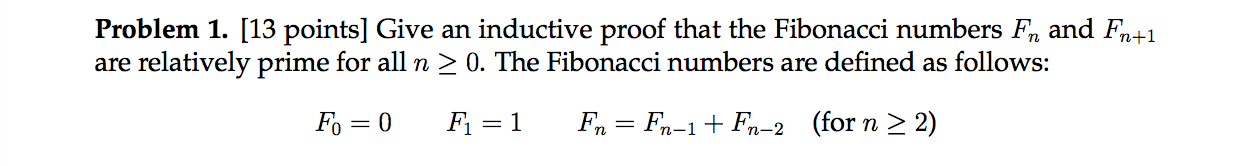
\includegraphics[width=400pt]{img/MIT-math-for-cs-2004-1.png}
\end{mdframed}

\begin{definition*}
  Integers $m$ and $n$ are relatively prime (coprime) if they have no common factors other than 1.
\end{definition*}


\begin{proof}
  $F_0 = 0$ and $F_1 = 1$ are coprime.

  Let $i > 1$ and suppose that $F_{i}$ and $F_{i+1}$ are coprime.

  We want to show that $F_{i+1}$ and $F_{i+2}$ are coprime.

  Suppose for a contradiction that $F_{i+1}$ and $F_{i+2}$ are not coprime.

  Then there exists $p, s \geq 1$ and $q > 1$ such that $F_{i+1} = pq$ and $F_{i+2} = sq$.

  Note that $F_{i+2} = sq = F_{i} + F_{i+1} = F_i + pq$, therefore $F_i = (s - p)q$, therefore
  $q$ is a factor of $F_i$, as well as of $F_{i+1}$.

  But by the inductive hypothesis, $F_{i}$ and $F_{i+1}$ are coprime, so $q$ cannot be a factor of
  both.

  This contradiction proves that $F_{i+1}$ and $F_{i+2}$ are coprime and, by induction, that the
  Fibonacci numbers $F_n$ and $F_{n+1}$ are coprime for all $n \geq 0$.


\end{proof}

% \begin{mdframed}
% 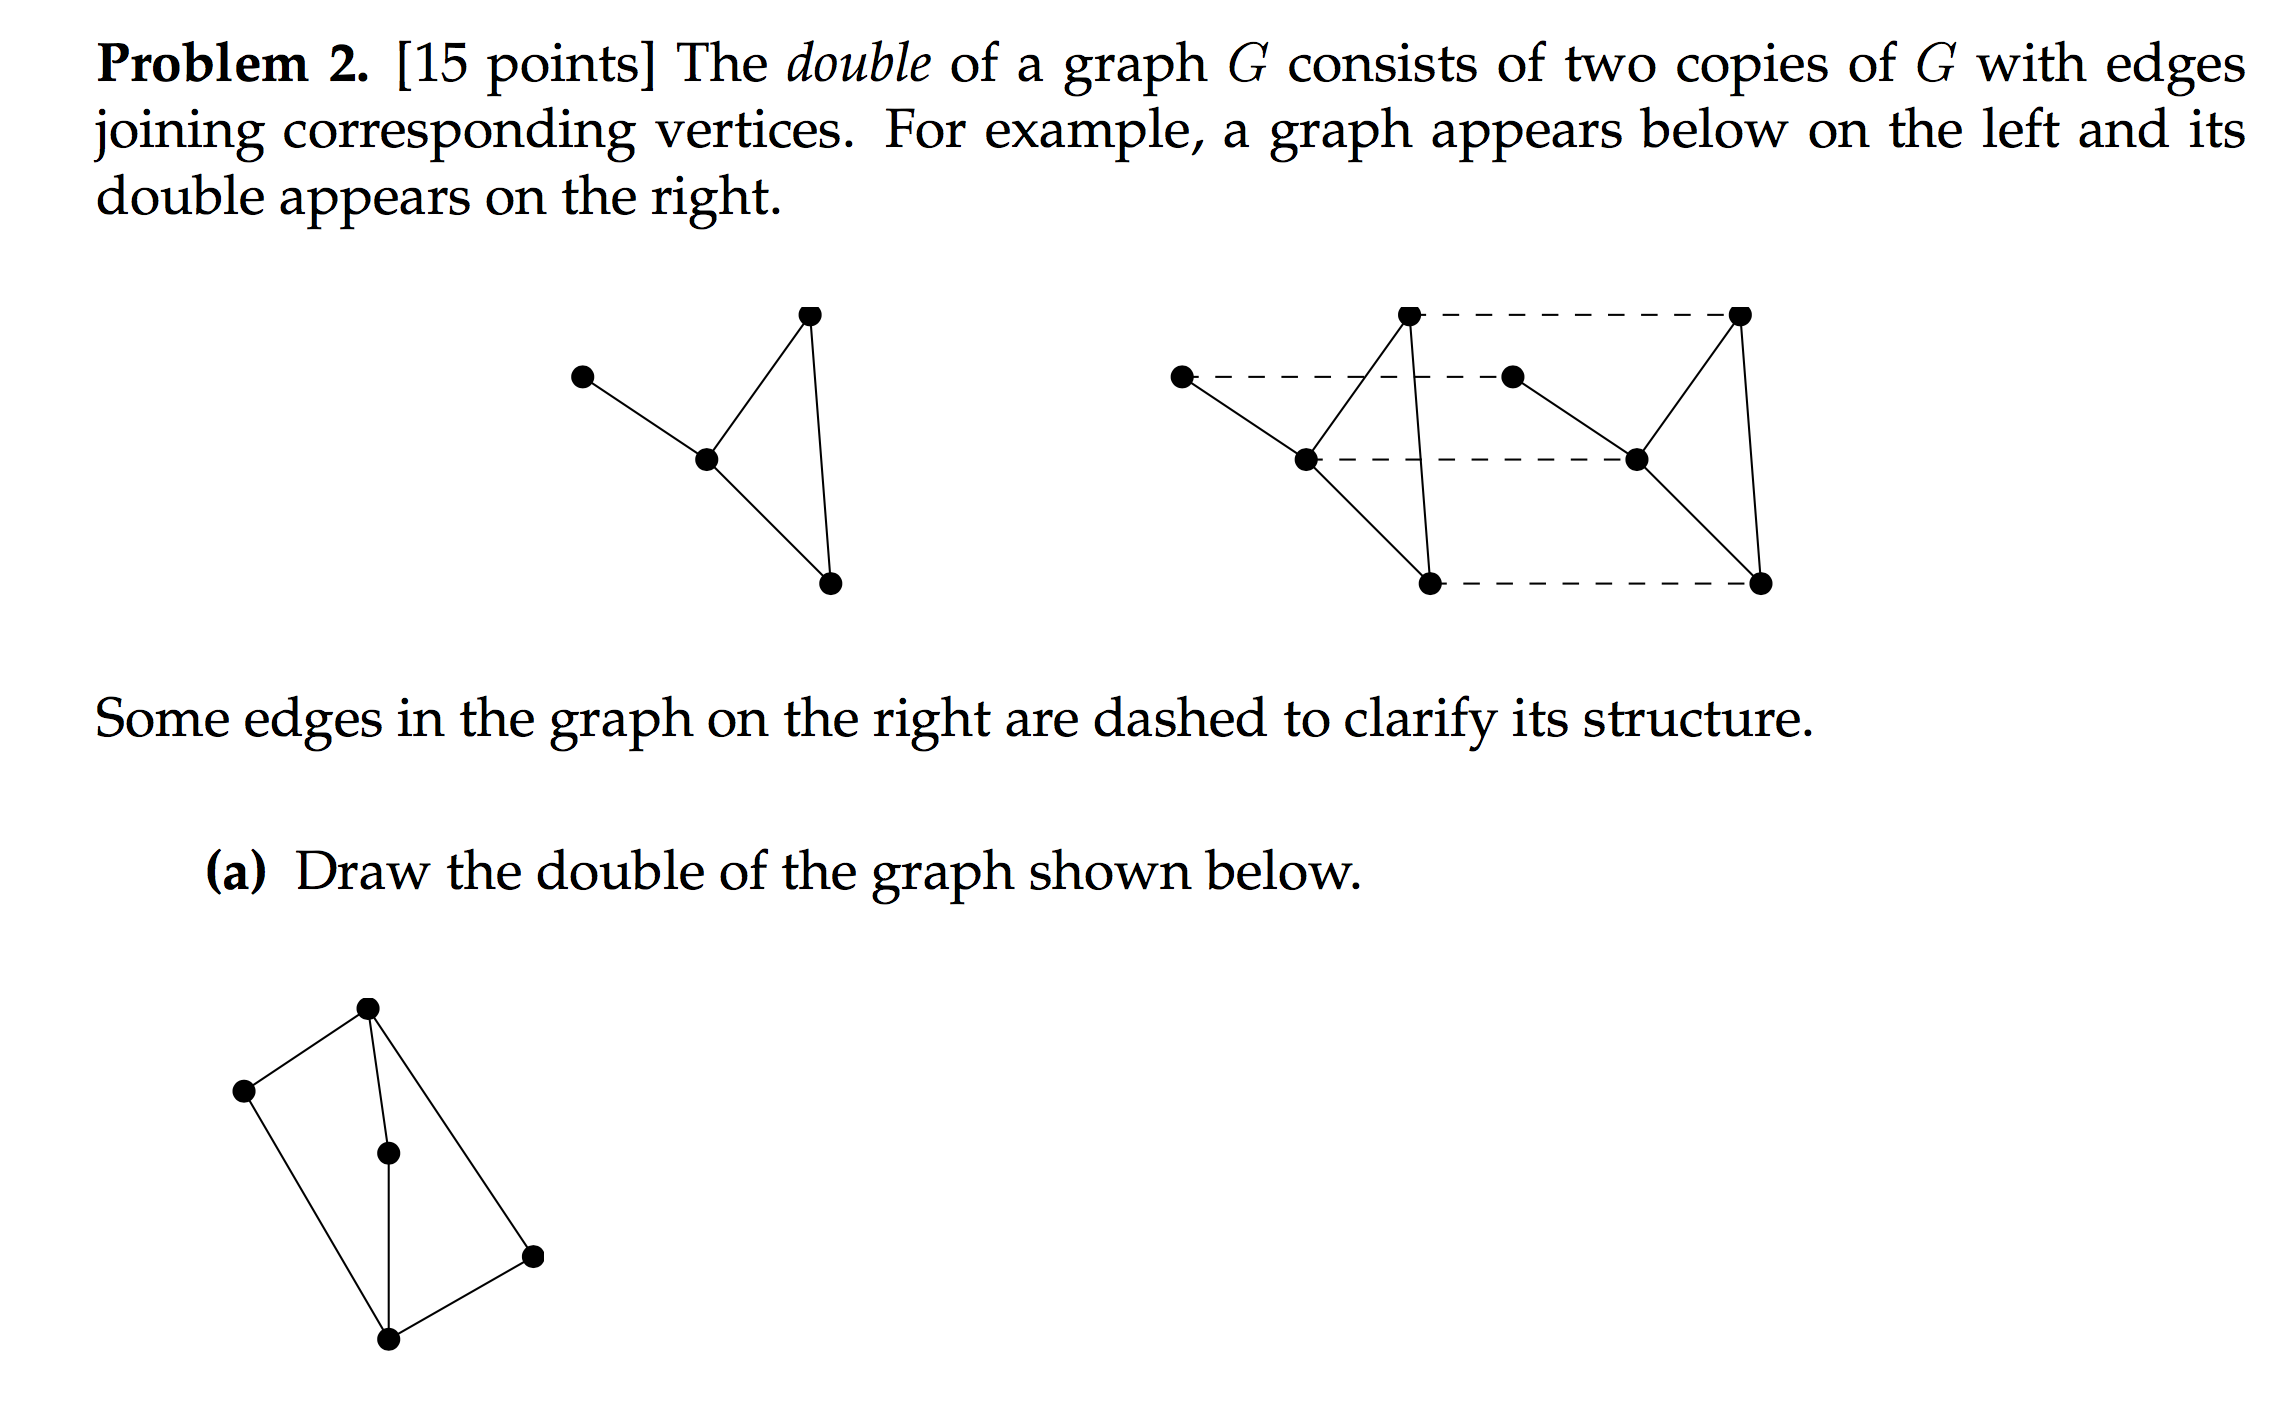
\includegraphics[width=400pt]{img/MIT-math-for-cs-2004-2-1.png}
% \end{mdframed}

% \begin{mdframed}
% 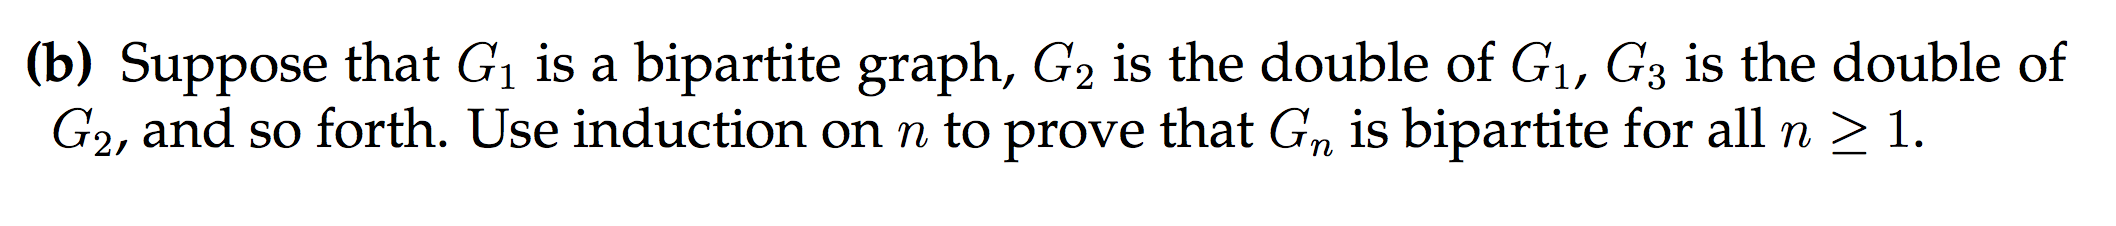
\includegraphics[width=400pt]{img/MIT-math-for-cs-2004-2-2.png}
% \end{mdframed}

% \begin{mdframed}
% 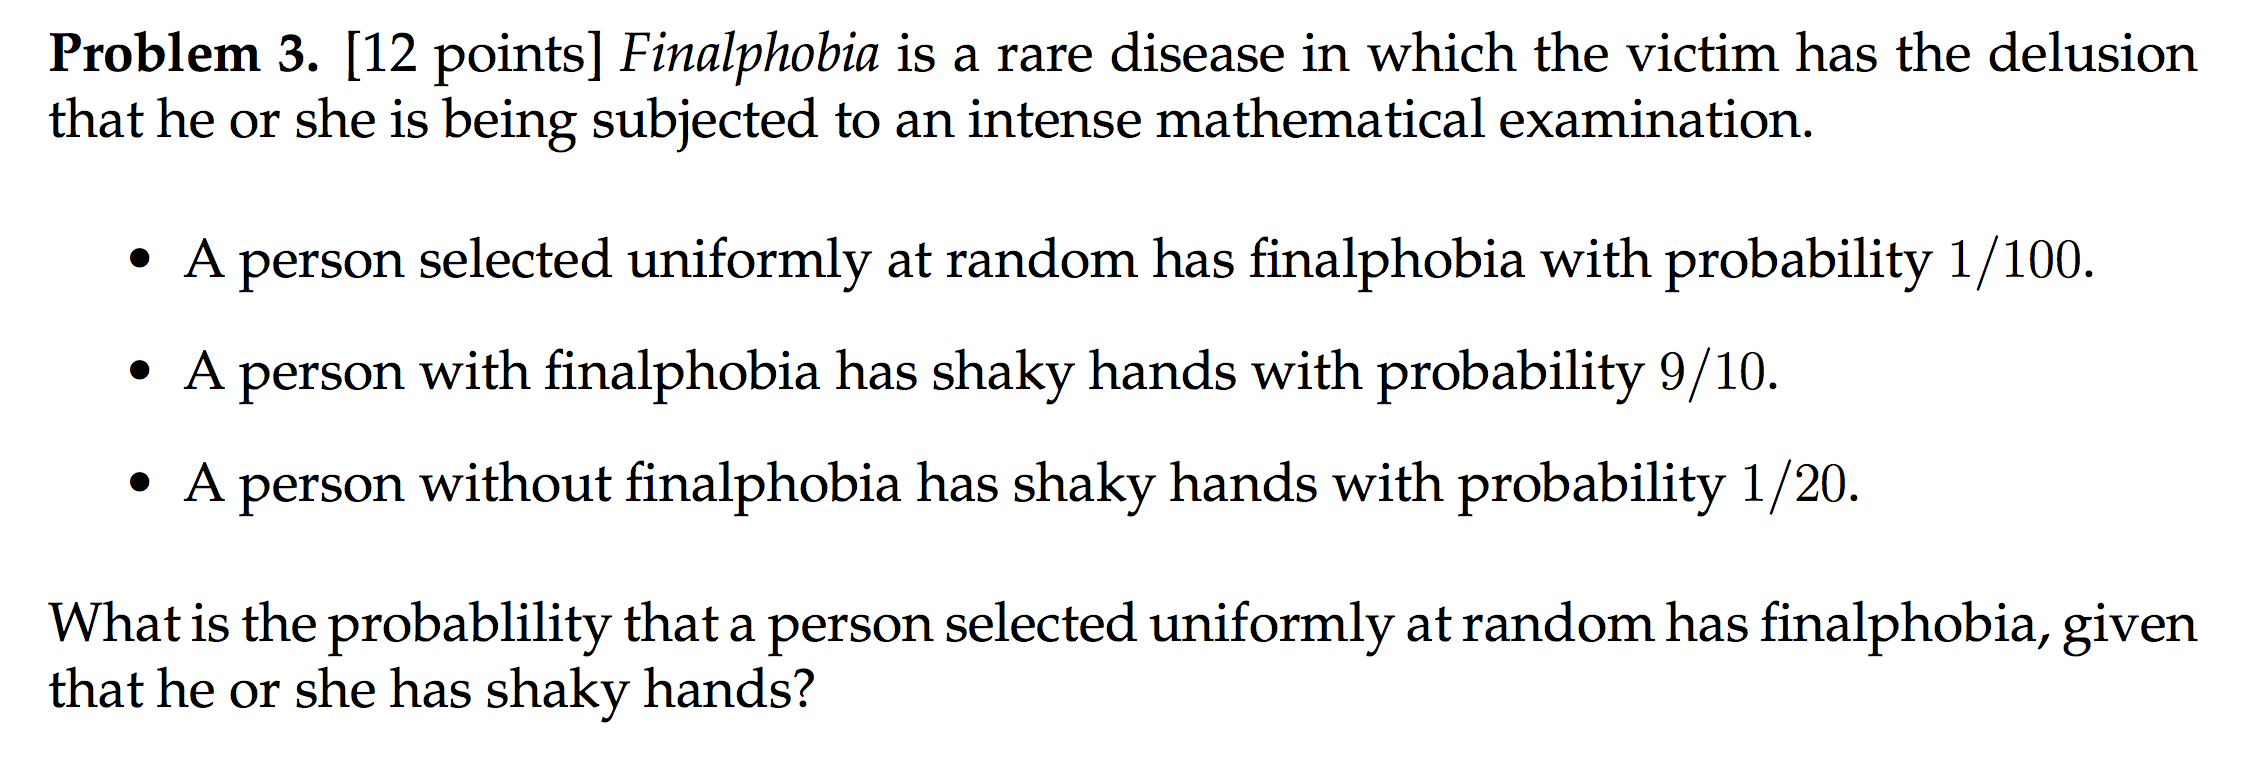
\includegraphics[width=400pt]{img/MIT-math-for-cs-2004-3.png}
% \end{mdframed}

\newpage
\begin{mdframed}

\includegraphics[width=400pt]{img/MIT-math-for-cs-2006-1.png}
\end{mdframed}
\begin{align*}
  \sumin i^2 = 1^2 + 2^2 + \ldots + n^2
\end{align*}

...induction.

\newpage
\begin{mdframed}
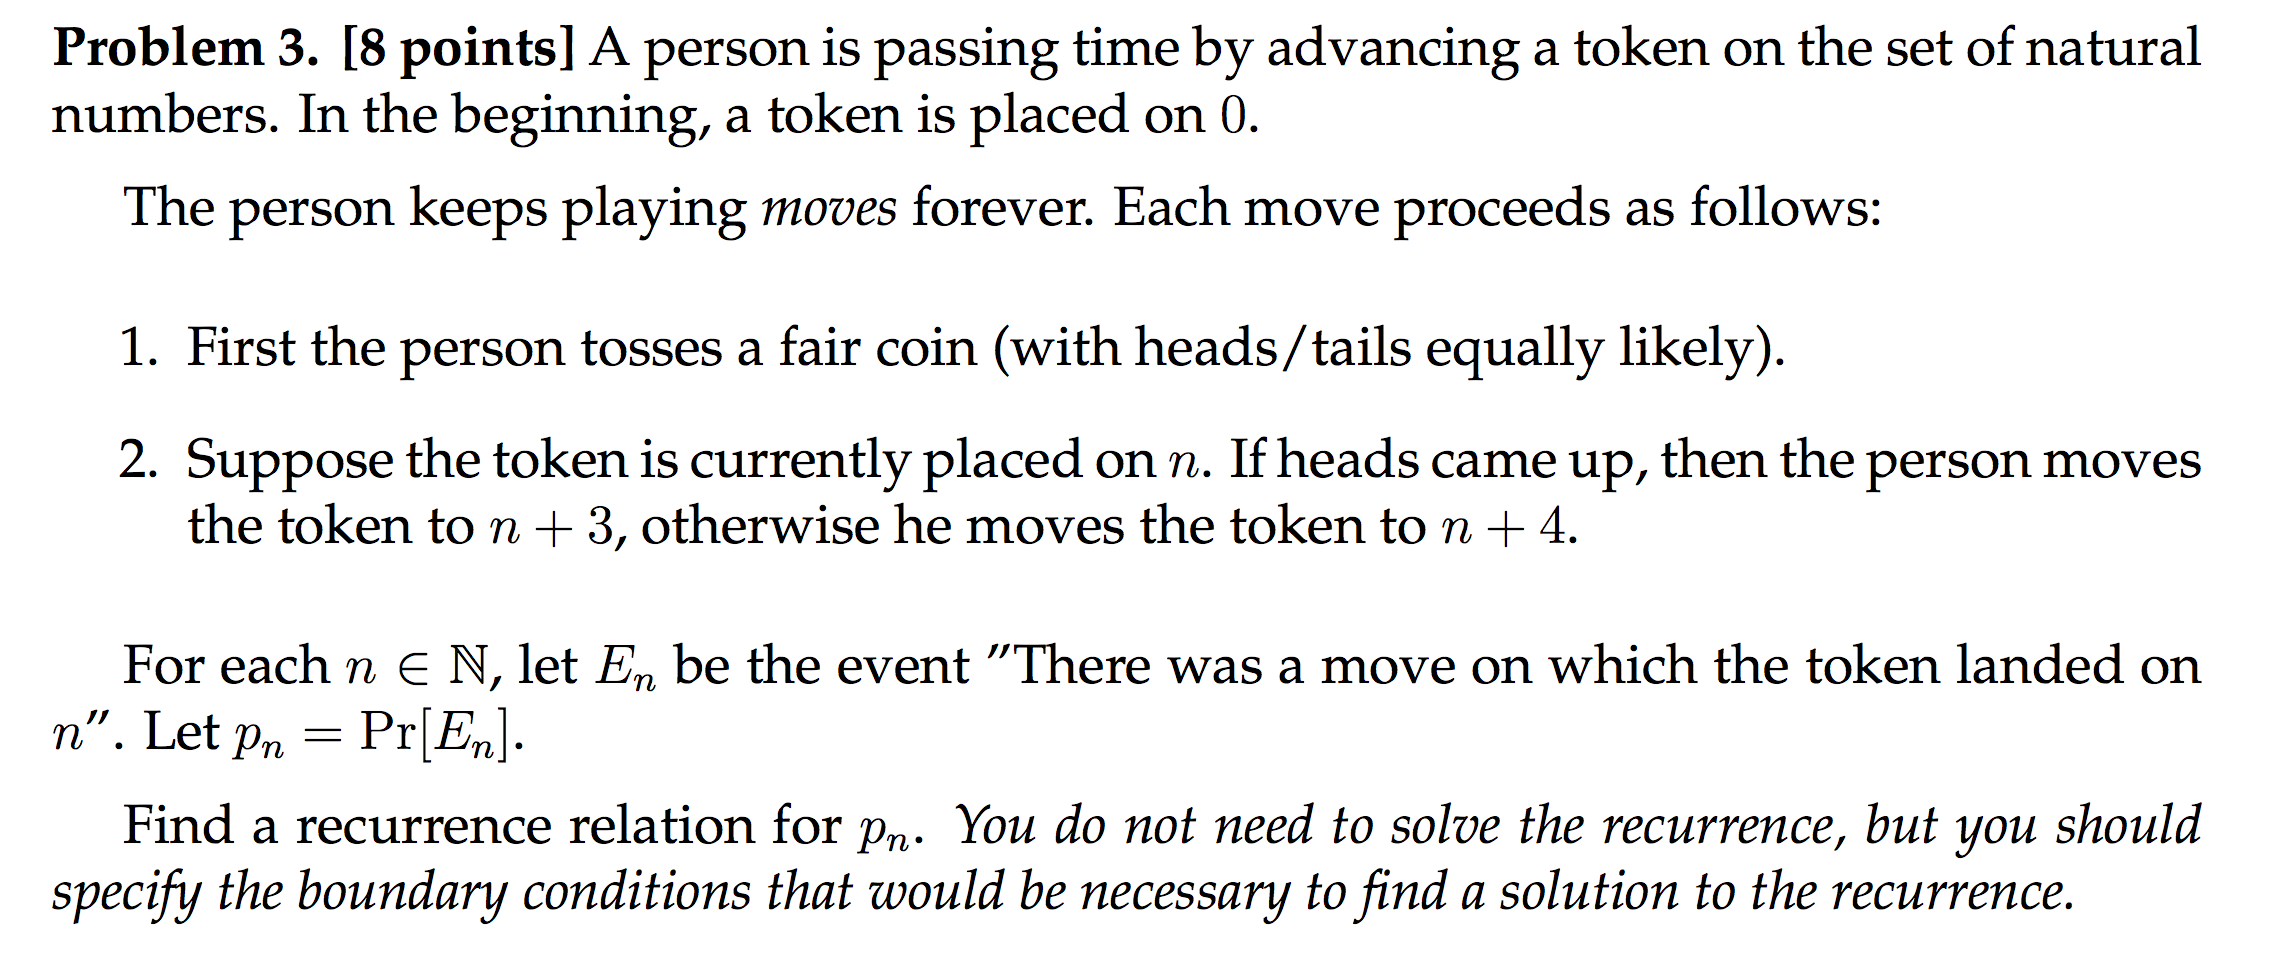
\includegraphics[width=400pt]{img/MIT-math-for-cs-2006-3.png}
\end{mdframed}
$p_0 = 1$\\
$p(1) = p(2) = 0$\\
$p(3) = \frac{1}{2}$\\
$p_n = \frac{1}{2}p_{n-3} + \frac{1}{2}p_{n-4}$ for $n \geq 4$\\

\newpage
\begin{mdframed}
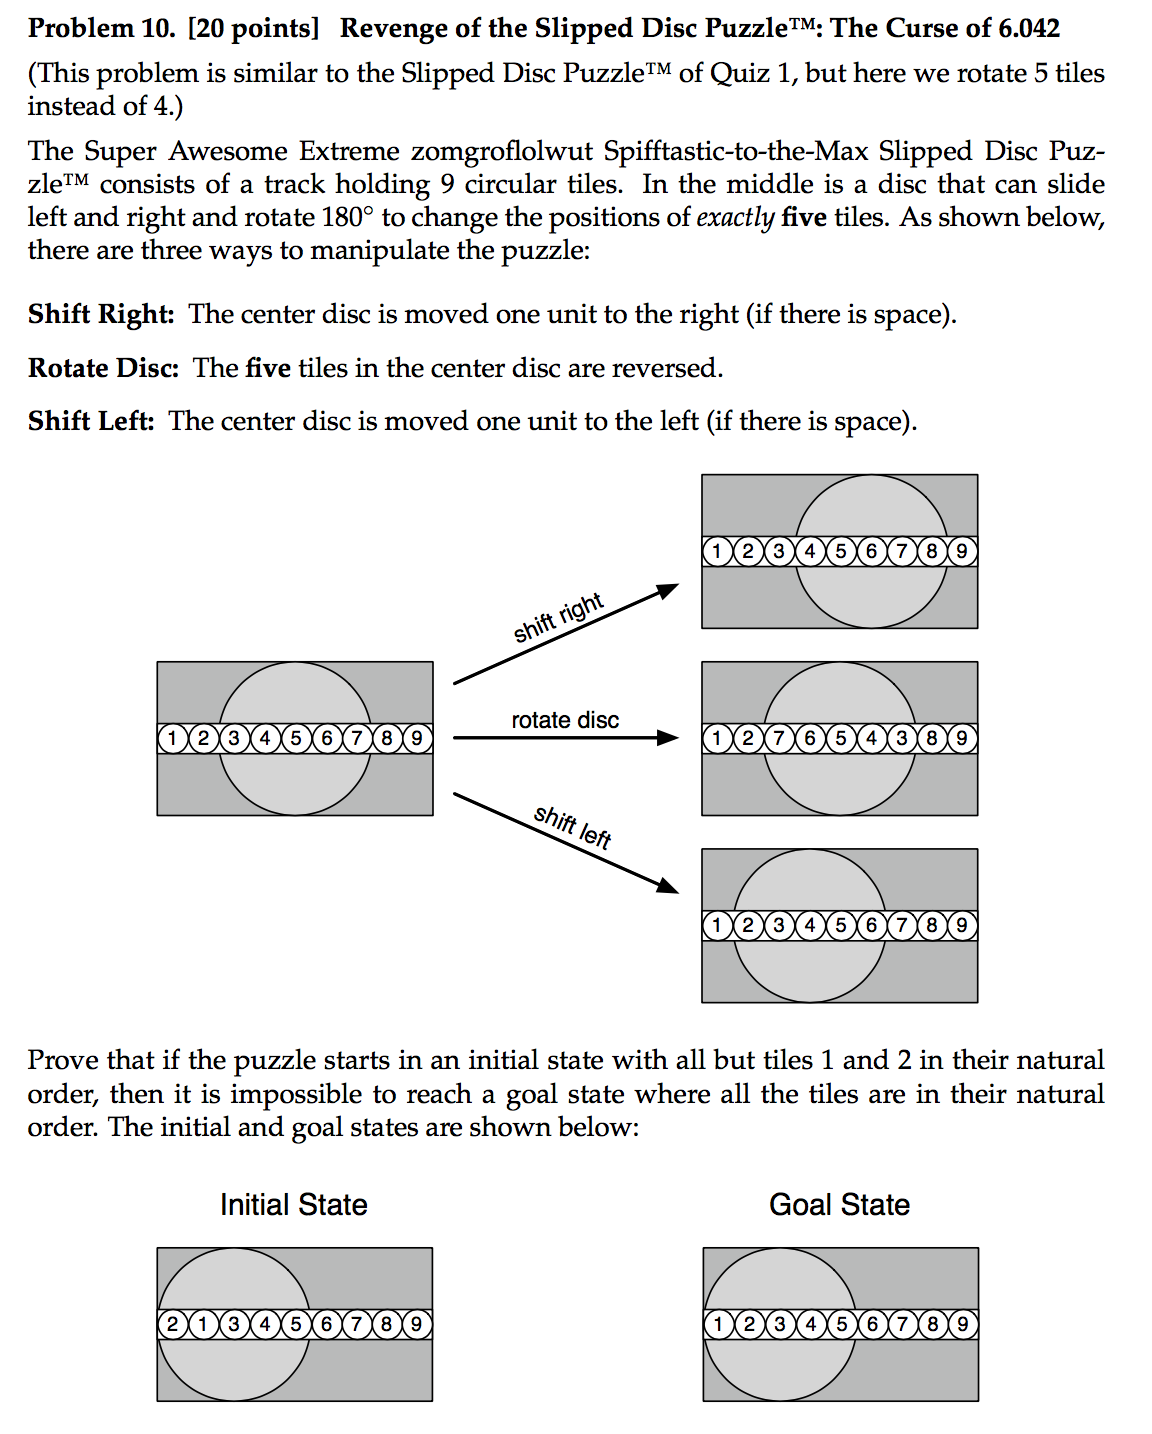
\includegraphics[width=400pt]{img/MIT-math-for-cs-2008-10.png}
\end{mdframed}

Let the positions be $1, 2, \ldots 9$.

Define the position of the dic to be the leftmost position that is under the disc. Therefore the
disc starts in position 1.

Note that every rotation affects 4 tiles and leaves 5 unchanged.

Suppose we can reach the goal state.

Then the last move is a rotation.

Note that we must perform a rotate move with the disc in position 1, since we must change the
position of the tile labeled 2 that starts in position 1.

\end{document}
